\documentclass{article}
\usepackage{amsmath}
\usepackage{amsfonts}
\usepackage{graphicx}
\title{Modeling Corruption in America using the Bush and Obama Administration}
\author{Joshua Wollenweber}

\begin{document}
\maketitle

	\begin{abstract}
	This paper intends to model corruption in the United States of America through a variation of the universal model of interraction (Lotka-Volterra). The model uses logistic decay of corruption and assumes that the new presidential administration interacts with the policies and achievements of the old administration. Data from the Obama and Bush presidential administrations were used as they directly follow each other chronologically. This interraction is assumed to affect the corruption level of the nation. Solution curves were created using a global and local carrying capacity, but yielded no significant difference. The model was determined to be ineffective at forecasting corruption levels in the United States.
	\end{abstract}

	\newpage
	\section{Introduction}
	\paragraph{}
	The goal of this project was to find a suitable model for forecasting corruption in the United States of America. To measure corruption, the Corruption Perception Index (CPI) was used from Transparency.org.
	\paragraph{}
	Transparency.org attempts to measure the perception of corruption in the public sector by consolidating and normalizing data from surveys by several big data businesses, which give their own measure of corruption. CPI has been measured in a rapidly increasing number of countries around the world since 1995. The CPI in the US has been measured from 1995 until their most recent report for 2018. 
	\paragraph{}
	Corruption can also be understood as the abuse of power, and presidential administrations demonstrate their abuse of power through their actions during term. Many of these actions may be self-serving (corrupt) and conflict (compete) with the policies and achievements of the administration preceding them. Therefore, the universal model of interaction will be used in attempts to model corruption within the US.

	\section{Methods}
		\subsection{Determining the Model}
		The CPI data for the US is shown with a trend-fitting curve in Figure \ref{USA CPI}. It is important to note the oscillitory nature of its change throughout the years.	
		\begin{figure}[h]
		\centering
		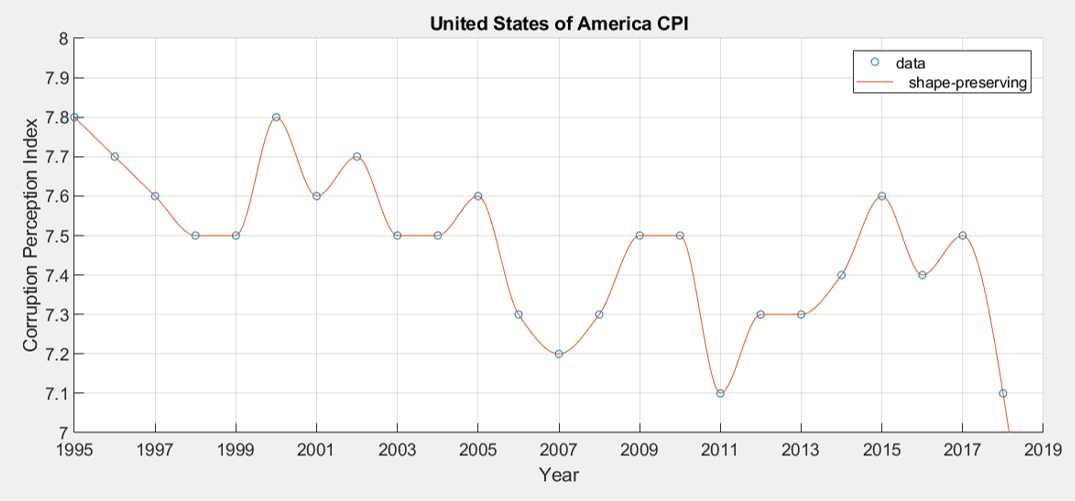
\includegraphics[width=1\textwidth]{USA_CPI}
		\caption{Shows the CPI score of the US from 1995 to 2018 with a lower bound of 7 and an upper bound of 8}
		\label{USA CPI}
		\end{figure}

		\paragraph{}
		Because of the oscillations in CPI throughout the years, it is important to fit the data to a growth/decay model. The nature of change in CPI must be indentified in order to determine the best model to use for this project. Logistic growth was tested, and Figure \ref{Logistic Fit} shows the data to fit logistic decay.
		\begin{figure}[h]
		\centering
		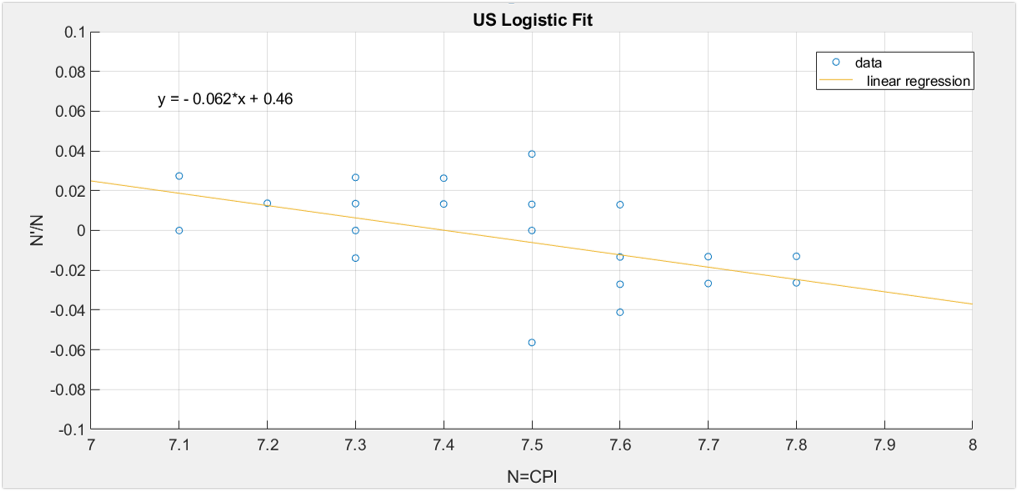
\includegraphics[width=1\textwidth]{logistic_fit}
		\caption{Shows the fit of US CPI data to a logistic decay model of growth. Noting the y-intercept identifies the global carrying capacity K to be 7.4194.}
		\label{Logistic Fit}
		\end{figure}


		\subsection{Model}
		\paragraph{}
		With this information, the following model was produced using four assumptions.
		\begin{enumerate}
		\item The change in CPI of the current (new) presidential administration is affected by the CPI of the previous (old) presidential administration.
		\item There is logistic decay in the change in CPI for any administration in the US.
		\item The CPI will go through logistic growth if the administration is corrupt, and will go through logistic decay if the administration is non-corrupt (coefficients a and m).
		\item The CPI will decrease if the new administration takes measures to deface or remove achievements/policies created by the old administration (coefficients b and n).
		\end{enumerate}
		\paragraph{}
		The universal model of interaction was used, which is a variation of the Lotka-Volterra equation. The Obama administration (2009-2016) is identified as the new administration, x, and the Bush administration (2001-2008) is identified as the old administration, y.
		\begin{equation}
		x'=x(-a(1-\frac{x}{K})-by)
		\end{equation}
		\begin{equation}
		y'=y(-m(1-\frac{y}{K})-nx)
		\end{equation}
		

		\subsection{Coefficients}
		\paragraph{}
		Coefficients were determined using the initial conditions for each administration. MatLab code was used to calculate these values, and the following equations were used. 
		\begin{equation}
		C_{x} = \ln{\frac{x_{0}}{x_{0}-K}}
		\end{equation}
		\begin{equation}
		C_{y} = \ln{\frac{y_{0}}{y_{0}-K}}
		\end{equation}
		\begin{equation}
		a = -\ln{\frac{K+x_{1}}{x_{1}}+C}
		\end{equation}
		\begin{equation}
		m = -\ln{\frac{K+y_{1}}{y_{1}}+C}
		\end{equation}
		\begin{equation}
		b = \frac{-x'-x(a(1-\frac{x}{K})}{x*y}
		\end{equation}
		\begin{equation}
		n = \frac{-y'-y(m(1-\frac{y}{K})}{x*y}
		\end{equation}
		\paragraph{}
		While the global carrying capacity, K, was used in the initial test of the model, local carrying capacities for each administration were calculated. The following equations were used for their calculation.
		\begin{equation}
		K_{x} = x_{1} * \frac{2*x_{0}*x_{2}-x_{0}*x_{1}-x_{1}*x_{2}}{x_{0}*x_{2}-x_{1}*x_{1}}
		\end{equation}	
		\begin{equation}
		K_{y} = y_{1} * \frac{2*y_{0}*y_{2}-y_{0}*y_{1}-y_{1}*y_{2}}{y_{0}*y_{2}-y_{1}*y_{1}}
		\end{equation}	

	\section{Results}
	\paragraph{}
	The nullclines for x' and y' were determined to gain an expectation for the results. This is shown in Figure \ref{Phase Portrait}.
	\begin{figure}[h]
	\centering
	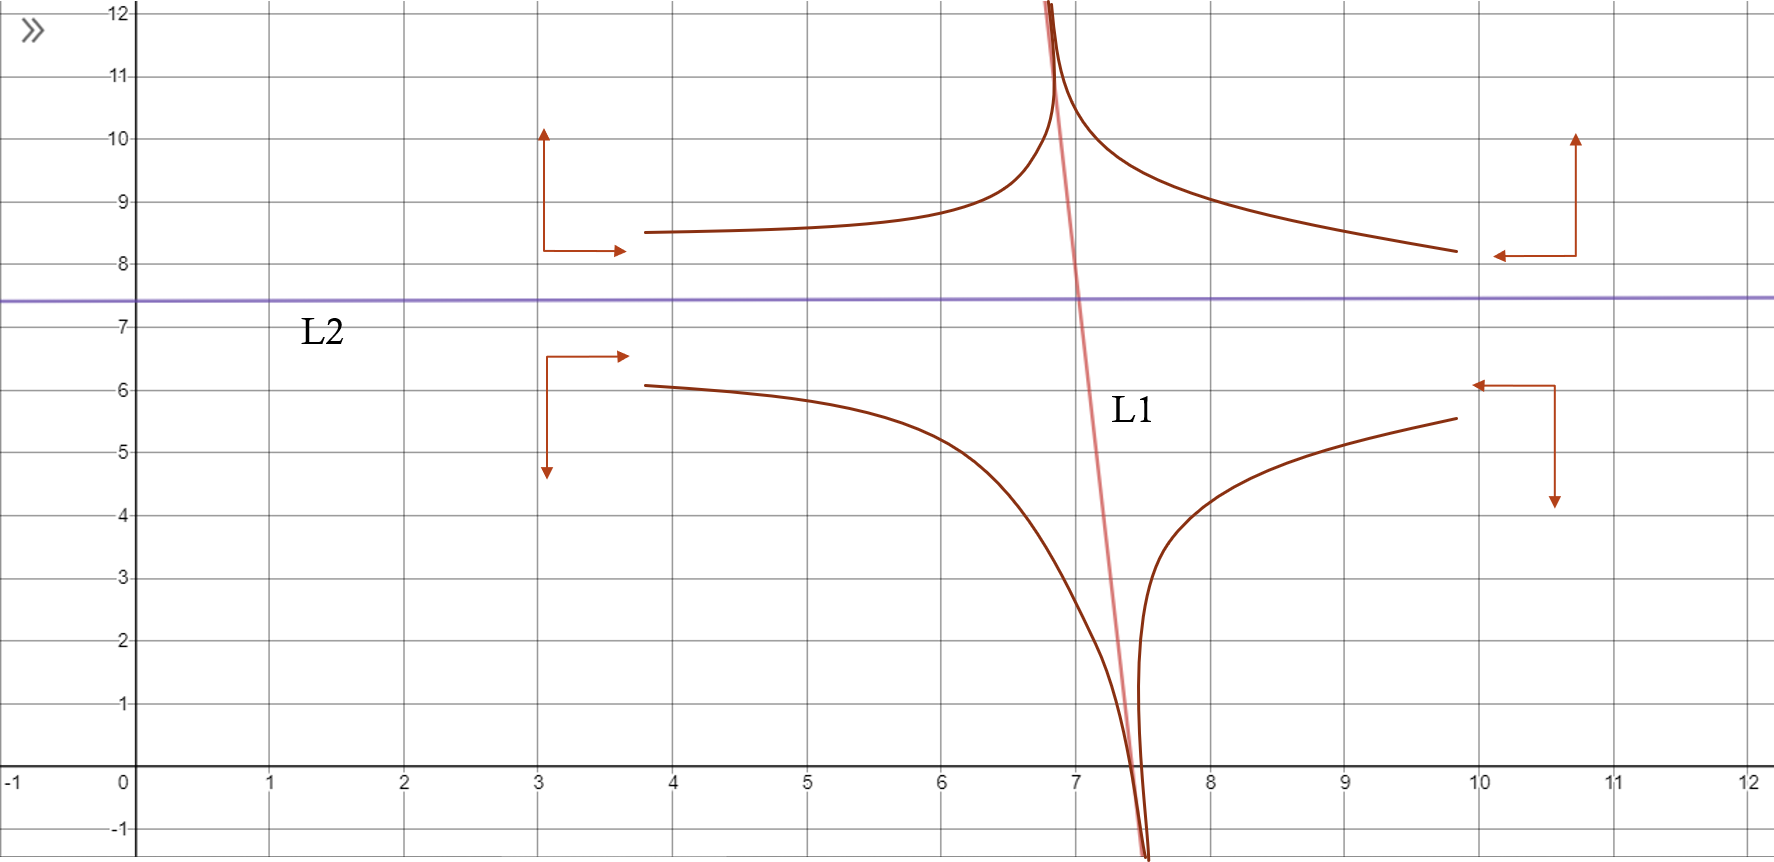
\includegraphics[width=1\textwidth]{phase_portrait}
	\caption{Shows the phase portrait of the model equations. L1 denotes the nullcline for the Obama administration. L2 denotes the nullcline for the Bush administration. Trajectories are shown in mahogany.}
	\label{Phase Portrait}
	\end{figure}

	\paragraph{}
	The phase portrait and solution curves are shown in Figure \ref{Solution1}. The solution curves show slight oscillation around their equillibrium points. These curves predict the CPI up to 10 years after the initial year. This graph uses the universal carrying capacity value of 7.4194. The Obama administration reaches an equillibrium at a CPI of 7, and the Bush administration reaches an equillibrium at a CPI of 7.5.
	\begin{figure}[!]
	\centering
	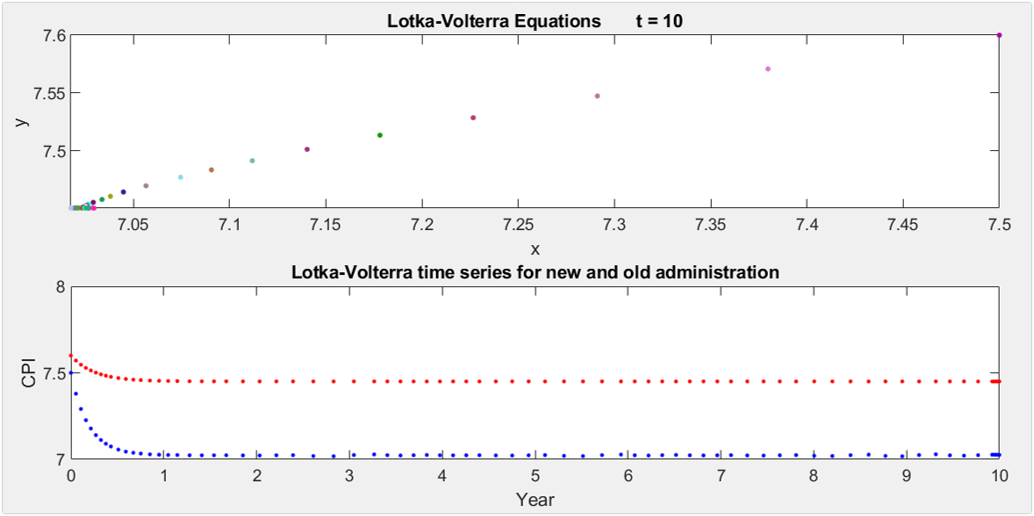
\includegraphics[width=1\textwidth]{solution_universal_k}
	\caption{The top graphics shows the phase portait as it oscillates around (7, 7.45). The bottom graphic shows the solutions of x (blue) and y (red)}
	\label{Solution1}
	\end{figure}

	\paragraph{}
	Another test using local carrying capacites from equations (9) and (10) is shown in Figure \ref{Solution2}. This shows no significant difference from Figure \ref{Solution1}, but there is slightly more oscillation about the equillibrium point (7, 7.45).
	\begin{figure}[!]
	\centering
	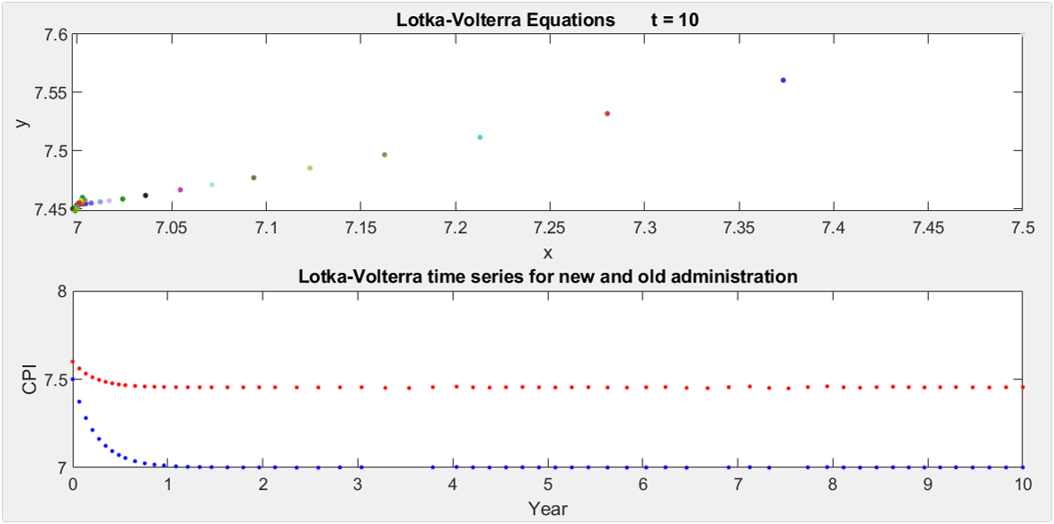
\includegraphics[width=1\textwidth]{solution_local_k}
	\caption{The top graphics shows the phase portait as it oscillates around (7, 7.45). The bottom graphic shows the solutions of x (blue) and y (red)}
	\label{Solution2}
	\end{figure}

	\paragraph{}
	Other approaches not displayed include: changing the initial conditions to the second and third year of a president's administration, experimenting with the values of a,n and b,m. It was determined that a and n must be negative for the solution curves to converge to a CPI value, that the initial conditions have an extremely varying effect on the equillibrium point on the solution curves, and positive b and m will yield an increasing solution curve that reaches an equillibrium while a negative b and m will yield a decreasing solution curve that reaches an equillibrium. The slight oscillation in the solution curves shown in Figures \ref{Solution1} and \ref{Solution2} was the most oscillation seen in any trials.

	\section{Conclusions}
	\paragraph{}
	It is clear that neither solution curves match with the actual trend shown in Figure \ref{USA CPI}. It is therefore clear that this model fails to accurately forecast the CPI in the US for any years after its initial condition. In order to improve the accuracy and effectiveness of the model, several steps can be taken.
	\begin{enumerate}
	\item Find a fit better than logistic decay. Figure \ref{Logistic Fit} demonstrates that the data does fit logistic decay, but it also clearly shows that the fit is poor, and may be coincidental.
	\item Improve interaction term with coefficients b and m. This term is likely too simple to model the complexity of this problem, and should model the real-world impact of postive-negative interaction between administrations more accurately.
	\end{enumerate}
	It is not clear yet to say that the universal model of interaction is a poor skeleton to use for this problem. This model's assumptions seem to correctly interpret the trend CPI would have given competitive vs cooperative administrations. The model's terms have not accurately portraited the complexity of the problem, and additions to the current assumptions should be made.

\end{document}